\documentclass[10pt,fleqn]{article} % Default font size and left-justified equations
\usepackage[%
    pdftitle={Informatique : Bases de données},
    pdfauthor={Xavier Pessoles}]{hyperref}

%%%%%%%%%%%%%%%%%%%%%%%%%%%%%%%%%%%%%%%%%
% Original author:
% Mathias Legrand (legrand.mathias@gmail.com) with modifications by:
% Vel (vel@latextemplates.com)
% License:
% CC BY-NC-SA 3.0 (http://creativecommons.org\newtheorem{rappelT}{Rappel}[section]/licenses/by-nc-sa/3.0/)
%%%%%%%%%%%%%%%%%%%%%%%%%%%%%%%%%%%%%%%%%

%----------------------------------------------------------------------------------------
%	VARIOUS REQUIRED PACKAGES AND CONFIGURATIONS
%----------------------------------------------------------------------------------------

\usepackage[top=2.5cm,bottom=2cm,left=2cm,right=2cm,headsep=40pt,a4paper]{geometry} % Page margins

\usepackage{graphicx} % Required for including pictures
\graphicspath{{images/}} % Specifies the directory where pictures are stored
\usepackage{float}

\usepackage{lipsum} % Inserts dummy text

\usepackage{tikz} % Required for drawing custom shapes

\usepackage[french]{babel} % English language/hyphenation
\frenchbsetup{StandardLists=true} % Pour éviter la collision babel enumitem pour les listes

\usepackage{enumitem} % Customize lists
\setlist{nolistsep} % Reduce spacing between bullet points and numbered lists

\usepackage{booktabs} % Required for nicer horizontal rules in tables

\usepackage{colortbl} % Couleur dans les tableaux

\usepackage{xcolor} % Required for specifying colors by name
%\definecolor{ocre}{RGB}{243,102,25} % Define the orange color used for highlighting throughout the book
\definecolor{ocre}{RGB}{49,133,156} % Couleur ''bleue''
\definecolor{violetf}{RGB}{112,48,160} % Couleur ''violet''
\usepackage{enumitem}
\usepackage{pifont} % Pour les dinglist
\usepackage{multicol}
\usepackage{array} % Centrage vertical dans les tableaux

%----------------------------------------------------------------------------------------
%	FONTS
%----------------------------------------------------------------------------------------

\usepackage{avant} % Use the Avantgarde font for headings
%\usepackage{times} % Use the Times font for headings
%\usepackage{mathptmx} % Use the Adobe Times Roman as the default text font together with math symbols from the Sym­bol, Chancery and Com­puter Modern fonts
\usepackage[adobe-utopia]{mathdesign}
\usepackage{microtype} % Slightly tweak font spacing for aesthetics
\usepackage[utf8]{inputenc} % Required for including letters with accents
\usepackage[T1]{fontenc} % Use 8-bit encoding that has 256 glyphs

%----------------------------------------------------------------------------------------
%	BIBLIOGRAPHY AND INDEX
%----------------------------------------------------------------------------------------

\usepackage[style=alphabetic,citestyle=numeric,sorting=nyt,sortcites=true,autopunct=true,babel=hyphen,hyperref=true,abbreviate=false,backref=true,backend=biber]{biblatex}
\addbibresource{bibliography.bib} % BibTeX bibliography file
\defbibheading{bibempty}{}

\usepackage{calc} % For simpler calculation - used for spacing the index letter headings correctly
\usepackage{makeidx} % Required to make an index
\makeindex % Tells LaTeX to create the files required for indexing

%----------------------------------------------------------------------------------------
%	MAIN TABLE OF CONTENTS
%----------------------------------------------------------------------------------------

\usepackage{titletoc} % Required for manipulating the table of contents

\setcounter{tocdepth}{2}     % Dans la table des matieres
\setcounter{secnumdepth}{2}

\contentsmargin{0cm} % Removes the default margin

% Part text styling
\titlecontents{part}[0cm]
{\addvspace{20pt}\centering\large\bfseries}
{}
{}
{}

% Chapter text styling
\titlecontents{chapter}[1.25cm] % Indentation
{\addvspace{12pt}\large\sffamily\bfseries} % Spacing and font options for chapters
{\color{ocre!60}\contentslabel[\Large\thecontentslabel]{1.25cm}\color{ocre}} % Chapter number
{\color{ocre}}  
{\color{ocre!60}\normalsize\;\titlerule*[.5pc]{.}\;\thecontentspage} % Page number

% Section text styling
\titlecontents{section}[1.25cm] % Indentation
{\addvspace{3pt}\sffamily\bfseries} % Spacing and font options for sections
{\color{ocre!60}\contentslabel[\thecontentslabel]{1.25cm} \color{ocre}} % Section number
{\color{ocre}}
{\hfill\color{ocre!60}\thecontentspage} % Page number
[]

% Subsection text styling
\titlecontents{subsection}[1.25cm] % Indentation
{\addvspace{1pt}\sffamily\small} % Spacing and font options for subsections
{\contentslabel[\thecontentslabel]{1.25cm}} % Subsection number
{}
{\ \titlerule*[.5pc]{.}\;\thecontentspage} % Page number
[]


% Subsection text styling
\titlecontents{subsubsection}[1.25cm] % Indentation
{\addvspace{1pt}\sffamily\small} % Spacing and font options for subsections
{\contentslabel[\thecontentslabel]{1.25cm}} % Subsection number
{}
{\ \titlerule*[.5pc]{.}\;\thecontentspage} % Page number
[]

% List of figures
\titlecontents{figure}[0em]
{\addvspace{-5pt}\sffamily}
{\thecontentslabel\hspace*{1em}}
{}
{\ \titlerule*[.5pc]{.}\;\thecontentspage}
[]

% List of tables
\titlecontents{table}[0em]
{\addvspace{-5pt}\sffamily}
{\thecontentslabel\hspace*{1em}}
{}
{\ \titlerule*[.5pc]{.}\;\thecontentspage}
[]

%----------------------------------------------------------------------------------------
%	MINI TABLE OF CONTENTS IN PART HEADS
%----------------------------------------------------------------------------------------

% Chapter text styling
\titlecontents{lchapter}[0em] % Indenting
{\addvspace{15pt}\large\sffamily\bfseries} % Spacing and font options for chapters
{\color{ocre}\contentslabel[\Large\thecontentslabel]{1.25cm}\color{ocre}} % Chapter number
{}  
{\color{ocre}\normalsize\sffamily\bfseries\;\titlerule*[.5pc]{.}\;\thecontentspage} % Page number

% Section text styling
\titlecontents{lsection}[0em] % Indenting
{\sffamily\small} % Spacing and font options for sections
{\contentslabel[\thecontentslabel]{1.25cm}} % Section number
{}
{}

% Subsection text styling
\titlecontents{lsubsection}[.5em] % Indentation
{\normalfont\footnotesize\sffamily} % Font settings
{}
{}
{}

%----------------------------------------------------------------------------------------
%	PAGE HEADERS
%----------------------------------------------------------------------------------------

\usepackage{fancyhdr} % Required for header and footer configuration



\pagestyle{fancy}
 \renewcommand{\headrulewidth}{0pt}
 \fancyhead{}
 \fancyhead[L]{%
 \noindent\begin{minipage}[c]{2.6cm}%
 
\includegraphics[width=2cm]{png/logo_lycee.png}%
 \end{minipage}}

\fancyhead[C]{\rule{8cm}{.5pt}}

 \fancyhead[R]{%
 \noindent\begin{minipage}[c]{3cm}
 \begin{flushright}
 \footnotesize{\textit{\textsf{\xxtete}}}%
 \end{flushright}
 \end{minipage}
}


\fancyfoot[C]{\rule{12cm}{.5pt}}
\renewcommand{\footrulewidth}{0.2pt}
\fancyfoot[C]{\footnotesize{\bfseries \thepage}}
\fancyfoot[L]{ 
\begin{minipage}[c]{.2\linewidth}
\noindent\footnotesize{{\xxauteur}}
\end{minipage}}


\fancyfoot[R]{\footnotesize{\xxpied}
\ifthenelse{\isodd{\value{page}}}{
\begin{tikzpicture}[overlay]
\node[shape=rectangle, 
      rounded corners = .25 cm,
	  draw= ocre,
	  line width=2pt, 
	  fill = ocre!10,
	  minimum width  = 2.5cm,
	  minimum height = 3cm,] at (\xxposongletx,\xxposonglety) {};
\node at (\xxposonglettext,\xxposonglety) {\rotatebox{90}{\textbf{\large\color{ocre}{\xxonglet}}}};
%{};
\end{tikzpicture}}{}
}
%
%
%
% Removes the header from odd empty pages at the end of chapters
\makeatletter
\renewcommand{\cleardoublepage}{
\clearpage\ifodd\c@page\else
\hbox{}
\vspace*{\fill}
\thispagestyle{empty}
\newpage
\fi}

\fancypagestyle{plain}{%
\fancyhf{} % vide l’en-tête et le pied~de~page.
%\fancyfoot[C]{\bfseries \thepage} % numéro de la page en cours en gras
% et centré en pied~de~page.
\fancyfoot[R]{\footnotesize{\xxpied}}
\fancyfoot[C]{\rule{12cm}{.5pt}}
\renewcommand{\footrulewidth}{0.2pt}
\fancyfoot[C]{\footnotesize{\bfseries \thepage}}
\fancyfoot[L]{ 
\begin{minipage}[c]{.2\linewidth}
\noindent\footnotesize{{\xxauteur}}
\end{minipage}}}



%----------------------------------------------------------------------------------------
%	THEOREM STYLES
%----------------------------------------------------------------------------------------

% Conflit avec la police adobe
%\usepackage{amsmath,amsfonts,amssymb,amsthm} % For math equations, theorems, symbols, etc
\usepackage{amsmath,amsthm}

\newcommand{\intoo}[2]{\mathopen{]}#1\,;#2\mathclose{[}}
\newcommand{\ud}{\mathop{\mathrm{{}d}}\mathopen{}}
\newcommand{\intff}[2]{\mathopen{[}#1\,;#2\mathclose{]}}
%\newtheorem{notation}{Notation}[chapter]
\newtheorem{notation}{Notation}[section]

% Boxed/framed environments
\newtheoremstyle{ocrenumbox}% % Theorem style name
{0pt}% Space above
{0pt}% Space below
{\normalfont}% % Body font
{}% Indent amount
{\small\bf\sffamily\color{ocre}}% % Theorem head font
{\;}% Punctuation after theorem head
{0.25em}% Space after theorem head
{\small\sffamily\color{ocre}\thmname{#1}\nobreakspace\thmnumber%{\@ifnotempty{#1}{}\@upn{#2}}% Theorem text (e.g. Theorem 2.1)
\thmnote{\nobreakspace\the\thm@notefont\sffamily\bfseries\color{black}---\nobreakspace#3.}} % Optional theorem note
\renewcommand{\qedsymbol}{$\blacksquare$}% Optional qed square


% Boite pour les corriges
\newtheoremstyle{correctionbox}% % Theorem style name
{0pt}% Space above
{0pt}% Space below
{\normalfont}% % Body font
{}% Indent amount
{\small\bf\sffamily\color{violet}}% % Theorem head font
{\;}% Punctuation after theorem head
{0.25em}% Space after theorem head
{\small\sffamily\color{ocre}\thmname{#1}\nobreakspace\thmnumber%{\@ifnotempty{#1}{}\@upn{#2}}% Theorem text (e.g. Theorem 2.1)
\thmnote{\nobreakspace\the\thm@notefont\sffamily\bfseries\color{black}---\nobreakspace#3.}} % Optional theorem note
\renewcommand{\qedsymbol}{$\blacksquare$}% Optional qed square



\newtheoremstyle{blacknumex}% Theorem style name
{5pt}% Space above
{5pt}% Space below
{\normalfont}% Body font
{} % Indent amount
{\small\bf\sffamily}% Theorem head font
{\;}% Punctuation after theorem head
{0.25em}% Space after theorem head
{\small\sffamily{\tiny\ensuremath{\blacksquare}}\nobreakspace\thmname{#1}\nobreakspace\thmnumber%{\@ifnotempty{#1}{}\@upn{#2}}% Theorem text (e.g. Theorem 2.1)
\thmnote{\nobreakspace\the\thm@notefont\sffamily\bfseries---\nobreakspace#3.}}% Optional theorem note

\newtheoremstyle{blacknumbox} % Theorem style name
{0pt}% Space above
{0pt}% Space below
{\normalfont}% Body font
{}% Indent amount
{\small\bf\sffamily}% Theorem head font
{\;}% Punctuation after theorem head
{0.25em}% Space after theorem head
{\small\sffamily\thmname{#1}\nobreakspace 
\thmnote{\nobreakspace\the\thm@notefont\sffamily\bfseries---\nobreakspace#3.}}% Optional theorem note

% Non-boxed/non-framed environments
\newtheoremstyle{ocrenum}% % Theorem style name
{5pt}% Space above
{5pt}% Space below
{\normalfont}% % Body font
{}% Indent amount
{\small\bf\sffamily\color{ocre}}% % Theorem head font
{\;}% Punctuation after theorem head
{0.25em}% Space after theorem head
{\small\sffamily\color{ocre}\thmname{#1}\nobreakspace%\thmnumber{\@ifnotempty{#1}{}\@upn{#2}}% Theorem text (e.g. Theorem 2.1)
\thmnote{\nobreakspace\the\thm@notefont\sffamily\bfseries\color{black}---\nobreakspace#3.}} % Optional theorem note
\renewcommand{\qedsymbol}{$\blacksquare$}% Optional qed square
\makeatother

% Environnement pour les titres de parties
\newtheoremstyle{partiebox} 
{0pt}% Space above
{0pt}% Space below
{\normalfont}% Body font
{}% Indent amount
{\small\bf\sffamily}% Theorem head font
{\;}% Punctuation after theorem head
{0.25em}% Space after theorem head




% Defines the theorem text style for each type of theorem to one of the three styles above
\newcounter{dummy} 
\numberwithin{dummy}{section}
\theoremstyle{ocrenumbox}
%\newtheorem{theoremeT}[dummy]{Théorème}
\newtheorem{theoremeT}[dummy]{Théorème}
\newtheorem{resultatT}[dummy]{Résultat}
\newtheorem{savoirT}[dummy]{Savoir}
\newtheorem{methodeT}[dummy]{Méthode}
\newtheorem{objectifT}[dummy]{Objectif}
%\newtheorem{problem}{Problem}[chapter]
\newtheorem{problem}{Problem}[section]
%\newtheorem{exerciseT}{Exercise}[chapter]
\newtheorem{exerciseT}{Exercice}[section]

\theoremstyle{blacknumex}
%\newtheorem{exampleT}{Example}[chapter]
\newtheorem{exempleT}{Exemple}[section]
\newtheorem{termT}{Terminal\\}[section]
\newtheorem{pyT}{Python\\}[section]
\newtheorem{sciT}{Scilab\\}[section]
\newtheorem{pseudoT}{Pseudo Code\\}[section]
\newtheorem{sqlT}{SQL\\}[section]

\theoremstyle{blacknumbox}
%\newtheorem{vocabulary}{Vocabulary}[chapter]
\newtheorem{vocabulary}{Vocabulaire}[section]
%\newtheorem{definitionT}{Definition}[section]
\newtheorem{definitionT}{Définition}[section]
\newtheorem{rappelT}{Rappel}[section]
\newtheorem{demoT}{Démonstration}[section]
\newtheorem{corollaryT}[dummy]{Corollaire}
\newtheorem{hypoT}{Hypothèse(s)}

\theoremstyle{ocrenum}
\newtheorem{proposition}[dummy]{Proposition}

\theoremstyle{partiebox}
\newtheorem{titrepartieT}[]{}
\newtheorem{titrechapitreT}[]{}

\theoremstyle{correctionbox}
\newtheorem{correctionT}[dummy]{\color{violet}{Correction}}

%----------------------------------------------------------------------------------------
%	DEFINITION OF COLORED BOXES
%----------------------------------------------------------------------------------------

\RequirePackage[framemethod=tikz]{mdframed} % Required for creating the theorem, definition, exercise and corollary boxes

% Theorem box
\newmdenv[skipabove=7pt,
skipbelow=7pt,
backgroundcolor=ocre!10,
linecolor=ocre,
innerleftmargin=5pt,
innerrightmargin=5pt,
innertopmargin=5pt,
leftmargin=0cm,
rightmargin=0cm,
innerbottommargin=5pt]{tBox}


% Correction
\newmdenv[skipabove=7pt,
skipbelow=7pt,
backgroundcolor=violet!10,
linecolor=violet,
innerleftmargin=5pt,
innerrightmargin=5pt,
innertopmargin=5pt,
leftmargin=0cm,
rightmargin=0cm,
innerbottommargin=5pt]{coBox}


% Exercise box	  
\newmdenv[skipabove=7pt,
skipbelow=7pt,
rightline=false,
leftline=true,
topline=false,
bottomline=false,
backgroundcolor=ocre!10,
linecolor=ocre,
innerleftmargin=5pt,
innerrightmargin=5pt,
innertopmargin=5pt,
innerbottommargin=5pt,
leftmargin=0cm,
rightmargin=0cm,
linewidth=4pt]{eBox}	

% Definition box
\newmdenv[skipabove=7pt,
skipbelow=7pt,
rightline=false,
leftline=true,
topline=false,
bottomline=false,
backgroundcolor=ocre!10,
linecolor=ocre,
innerleftmargin=5pt,
innerrightmargin=5pt,
innertopmargin=1pt,
leftmargin=0cm,
rightmargin=0cm,
linewidth=4pt,
innerbottommargin=0pt]{dBox}	

% Demonstration box
\newmdenv[skipabove=7pt,
skipbelow=7pt,
rightline=false,
leftline=true,
topline=false,
bottomline=false,
%backgroundcolor=ocre!10,
linecolor=ocre,
innerleftmargin=5pt,
innerrightmargin=5pt,
innertopmargin=0pt,
leftmargin=0cm,
rightmargin=0cm,
linewidth=4pt,
innerbottommargin=0pt]{demoBox}	

% Corollary box
\newmdenv[skipabove=7pt,
skipbelow=7pt,
rightline=false,
leftline=true,
topline=false,
bottomline=false,
linecolor=gray,
backgroundcolor=black!5,
innerleftmargin=5pt,
innerrightmargin=5pt,
innertopmargin=5pt,
leftmargin=0cm,
rightmargin=0cm,
linewidth=4pt,
innerbottommargin=5pt]{cBox}


% Hypothèses
\newmdenv[skipabove=7pt,
skipbelow=7pt,
rightline=false,
leftline=true,
topline=false,
bottomline=false,
linecolor=gray,
backgroundcolor=black!5,
innerleftmargin=5pt,
innerrightmargin=5pt,
innertopmargin=5pt,
leftmargin=0cm,
rightmargin=0cm,
linewidth=4pt,
innerbottommargin=5pt]{hyBox}


% Boite pour le titre de la partie (pBox)
\newmdenv[skipabove=7pt,
skipbelow=7pt,
rightline=true,
leftline=false,
topline=false,
bottomline=false,
linecolor=ocre,
backgroundcolor=none,
innerleftmargin=5pt,
innerrightmargin=5pt,
innertopmargin=5pt,
leftmargin=0cm,
rightmargin=0cm,
linewidth=4pt,
innerbottommargin=5pt]{pBox}

% Boite pour le titre du chapitre (chBox)
\newmdenv[skipabove=7pt,
skipbelow=7pt,
rightline=false,
leftline=true,
topline=false,
bottomline=false,
linecolor=ocre,
%backgroundcolor=black!5,
innerleftmargin=5pt,
innerrightmargin=5pt,
innertopmargin=5pt,
leftmargin=0cm,
rightmargin=0cm,
linewidth=4pt,
innerbottommargin=5pt]{chBox}


% Boite pour les exemples
\newmdenv[skipabove=7pt,
skipbelow=7pt,
rightline=false,
leftline=true,
topline=false,
bottomline=false,
linecolor=gray,
backgroundcolor=white,
innerleftmargin=5pt,
innerrightmargin=5pt,
innertopmargin=5pt,
leftmargin=0cm,
rightmargin=0cm,
linewidth=4pt,
innerbottommargin=5pt]{exBox}

% Boite pour le terminal
\newmdenv[skipabove=7pt,
skipbelow=7pt,
rightline=false,
leftline=true,
topline=false,
bottomline=false,
linecolor=gray,
backgroundcolor=white,
innerleftmargin=5pt,
innerrightmargin=5pt,
innertopmargin=5pt,
leftmargin=0cm,
rightmargin=0cm,
linewidth=4pt,
innerbottommargin=5pt]{termBox}


% Boite pour Python
\newmdenv[skipabove=7pt,
skipbelow=7pt,
rightline=false,
leftline=true,
topline=false,
bottomline=false,
linecolor=gray,
backgroundcolor=white,
innerleftmargin=5pt,
innerrightmargin=5pt,
innertopmargin=5pt,
leftmargin=0cm,
rightmargin=0cm,
linewidth=4pt,
innerbottommargin=5pt]{pyBox}

% Boite pour scilab
\newmdenv[skipabove=7pt,
skipbelow=7pt,
rightline=false,
leftline=true,
topline=false,
bottomline=false,
linecolor=gray,
backgroundcolor=white,
innerleftmargin=5pt,
innerrightmargin=5pt,
innertopmargin=5pt,
leftmargin=0cm,
rightmargin=0cm,
linewidth=4pt,
innerbottommargin=5pt]{sciBox}


% Boite pour pseudo
\newmdenv[skipabove=7pt,
skipbelow=7pt,
rightline=false,
leftline=true,
topline=false,
bottomline=false,
linecolor=gray,
backgroundcolor=white,
innerleftmargin=5pt,
innerrightmargin=5pt,
innertopmargin=5pt,
leftmargin=0cm,
rightmargin=0cm,
linewidth=4pt,
innerbottommargin=5pt]{pseudoBox}

% Boite pour pseudo
\newmdenv[skipabove=7pt,
skipbelow=7pt,
rightline=false,
leftline=true,
topline=false,
bottomline=false,
linecolor=gray,
backgroundcolor=white,
innerleftmargin=5pt,
innerrightmargin=5pt,
innertopmargin=5pt,
leftmargin=0cm,
rightmargin=0cm,
linewidth=4pt,
innerbottommargin=5pt]{sqlBox}


% Creates an environment for each type of theorem and assigns it a theorem text style from the "Theorem Styles" section above and a colored box from above
\newenvironment{theorem}{\begin{tBox}\begin{theoremeT}}{\end{theoremeT}\end{tBox}}
\newenvironment{resultat}{\begin{tBox}\begin{resultatT}}{\end{resultatT}\end{tBox}}
\newenvironment{methode}{\begin{tBox}\begin{methodeT}}{\end{methodeT}\end{tBox}}
\newenvironment{savoir}{\begin{tBox}\begin{savoirT}}{\end{savoirT}\end{tBox}}
\newenvironment{obj}{\begin{tBox}\begin{objectifT}}{\end{objectifT}\end{tBox}}
\newenvironment{corrige}{\begin{coBox}\begin{correctionT}}{\end{correctionT}\end{coBox}}
\newenvironment{exercise}{\begin{eBox}\begin{exerciseT}}{\hfill{\color{ocre}\tiny\ensuremath{\blacksquare}}\end{exerciseT}\end{eBox}}				  
\newenvironment{exercice}{\begin{eBox}\begin{exerciseT}}{\hfill{\color{ocre}\tiny\ensuremath{\blacksquare}}\end{exerciseT}\end{eBox}}				  

\newenvironment{definition}{\begin{dBox}\begin{definitionT}}{\end{definitionT}\end{dBox}}	
\newenvironment{defi}{\begin{dBox}\begin{definitionT}}{\end{definitionT}\end{dBox}}	
\newenvironment{demo}{\begin{demoBox}\begin{demoT}}{\end{demoT}\end{demoBox}}	
\newenvironment{rappel}{\begin{dBox}\begin{rappelT}}{\end{rappelT}\end{dBox}}	
%\newenvironment{exemple}{\begin{exempleT}}{\hfill{\tiny\ensuremath{\blacksquare}}\end{exempleT}}		
\newenvironment{corollary}{\begin{cBox}\begin{corollaryT}}{\end{corollaryT}\end{cBox}}
\newenvironment{hypo}{\begin{hyBox}\begin{hypoT}}{\end{hypoT}\end{hyBox}}	\newenvironment{exemple}{\begin{exBox}\begin{exempleT}}{\hfill{\tiny\ensuremath{\blacksquare}}\end{exempleT}\end{exBox}}	
\newenvironment{titrepartie}{\begin{pBox}\begin{titrepartieT}}{\end{titrepartieT}\end{pBox}}	
\newenvironment{titrechapitre}{\begin{chBox}\begin{titrechapitreT}}{\end{titrechapitreT}\end{chBox}}	

\newenvironment{term}{ \begin{termBox}\begin{termT}}{\end{termT}\end{termBox}}
\newenvironment{py}{ \begin{pyBox}\begin{pyT}}{\end{pyT}\end{pyBox}}
\newenvironment{sci}{ \begin{sciBox}\begin{sciT}}{\end{sciT}\end{sciBox}}
\newenvironment{pseudo}{ \begin{pseudoBox}\begin{pseudoT}}{\end{pseudoT}\end{pseudoBox}}
\newenvironment{envsql}{ \begin{sqlBox}\begin{sqlT}}{\end{sqlT}\end{sqlBox}}


%----------------------------------------------------------------------------------------
%	REMARK ENVIRONMENT
%----------------------------------------------------------------------------------------

\newenvironment{remark}{\par\vspace{10pt}\small % Vertical white space above the remark and smaller font size
\begin{list}{}{
\leftmargin=35pt % Indentation on the left
\rightmargin=25pt}\item\ignorespaces % Indentation on the right
\makebox[-2.5pt]{\begin{tikzpicture}[overlay]
\node[draw=ocre!60,line width=1pt,circle,fill=ocre!25,font=\sffamily\bfseries,inner sep=2pt,outer sep=0pt] at (-15pt,0pt){\textcolor{ocre}{R}};\end{tikzpicture}} % Orange R in a circle
\advance\baselineskip -1pt}{\end{list}\vskip5pt} % Tighter line spacing and white space after remark

\newenvironment{rem}{\par\vspace{10pt}\small % Vertical white space above the remark and smaller font size
\begin{list}{}{
\leftmargin=35pt % Indentation on the left
\rightmargin=25pt}\item\ignorespaces % Indentation on the right
\makebox[-2.5pt]{\begin{tikzpicture}[overlay]
\node[draw=ocre!60,line width=1pt,circle,fill=ocre!25,font=\sffamily\bfseries,inner sep=2pt,outer sep=0pt] at (-15pt,0pt){\textcolor{ocre}{R}};\end{tikzpicture}} % Orange R in a circle
\advance\baselineskip -1pt}{\end{list}\vskip5pt} % Tighter line spacing and white space after remark


\newenvironment{warn}{\par\vspace{10pt}\small % Vertical white space above the remark and smaller font size
\begin{list}{}{
\leftmargin=35pt % Indentation on the left
\rightmargin=25pt}\item\ignorespaces % Indentation on the right
\makebox[-2.5pt]{\begin{tikzpicture}[overlay]
\node[draw=red!60,line width=1pt,circle,fill=red!25,font=\sffamily\bfseries,inner sep=2pt,outer sep=0pt] at (-15pt,0pt){\textcolor{black}{!}};\end{tikzpicture}} % Point d'exclamation dans un cercle
\advance\baselineskip -1pt}{\end{list}\vskip5pt} % Tighter line spacing and white space after remark


%----------------------------------------------------------------------------------------
%	SECTION NUMBERING IN THE MARGIN
%----------------------------------------------------------------------------------------
\setcounter{secnumdepth}{3}
\setcounter{tocdepth}{2}



\makeatletter
\renewcommand{\@seccntformat}[1]{\llap{\textcolor{ocre}{\csname the#1\endcsname}\hspace{1em}}}                    
\renewcommand{\section}{\@startsection{section}{1}{\z@}
{-4ex \@plus -1ex \@minus -.4ex}
{1ex \@plus.2ex }
{\normalfont\large\sffamily\bfseries}}
\renewcommand{\subsection}{\@startsection {subsection}{2}{\z@}
{-3ex \@plus -0.1ex \@minus -.4ex}
{0.5ex \@plus.2ex }
{\normalfont\sffamily\bfseries}}
\renewcommand{\subsubsection}{\@startsection {subsubsection}{3}{\z@}
{-2ex \@plus -0.1ex \@minus -.2ex}
{.2ex \@plus.2ex }
{\normalfont\small\sffamily\bfseries}}                        
\renewcommand\paragraph{\@startsection{paragraph}{4}{\z@}
{-2ex \@plus-.2ex \@minus .2ex}
{.1ex}
{\normalfont\small\sffamily\bfseries}}

%----------------------------------------------------------------------------------------
%	PART HEADINGS
%----------------------------------------------------------------------------------------


%----------------------------------------------------------------------------------------
%	CHAPTER HEADINGS
%----------------------------------------------------------------------------------------

% \newcommand{\thechapterimage}{}%
% \newcommand{\chapterimage}[1]{\renewcommand{\thechapterimage}{#1}}%
% \def\@makechapterhead#1{%
% {\parindent \z@ \raggedright \normalfont
% \ifnum \c@secnumdepth >\m@ne
% \if@mainmatter
% \begin{tikzpicture}[remember picture,overlay]
% \node at (current page.north west)
% {\begin{tikzpicture}[remember picture,overlay]
% \node[anchor=north west,inner sep=0pt] at (0,0) {\includegraphics[width=\paperwidth]{\thechapterimage}};
% \draw[anchor=west] (\Gm@lmargin,-9cm) node [line width=2pt,rounded corners=15pt,draw=ocre,fill=white,fill opacity=0.5,inner sep=15pt]{\strut\makebox[22cm]{}};
% \draw[anchor=west] (\Gm@lmargin+.3cm,-9cm) node {\huge\sffamily\bfseries\color{black}\thechapter. #1\strut};
% \end{tikzpicture}};
% \end{tikzpicture}
% \else
% \begin{tikzpicture}[remember picture,overlay]
% \node at (current page.north west)
% {\begin{tikzpicture}[remember picture,overlay]
% \node[anchor=north west,inner sep=0pt] at (0,0) {\includegraphics[width=\paperwidth]{\thechapterimage}};
% \draw[anchor=west] (\Gm@lmargin,-9cm) node [line width=2pt,rounded corners=15pt,draw=ocre,fill=white,fill opacity=0.5,inner sep=15pt]{\strut\makebox[22cm]{}};
% \draw[anchor=west] (\Gm@lmargin+.3cm,-9cm) node {\huge\sffamily\bfseries\color{black}#1\strut};
% \end{tikzpicture}};
% \end{tikzpicture}
% \fi\fi\par\vspace*{270\p@}}}

%-------------------------------------------

\def\@makeschapterhead#1{%
\begin{tikzpicture}[remember picture,overlay]
\node at (current page.north west)
{\begin{tikzpicture}[remember picture,overlay]
\node[anchor=north west,inner sep=0pt] at (0,0) {\includegraphics[width=\paperwidth]{\thechapterimage}};
\draw[anchor=west] (\Gm@lmargin,-9cm) node [line width=2pt,rounded corners=15pt,draw=ocre,fill=white,fill opacity=0.5,inner sep=15pt]{\strut\makebox[22cm]{}};
\draw[anchor=west] (\Gm@lmargin+.3cm,-9cm) node {\huge\sffamily\bfseries\color{black}#1\strut};
\end{tikzpicture}};
\end{tikzpicture}
\par\vspace*{270\p@}}
\makeatother

%----------------------------------------------------------------------------------------
%	HYPERLINKS IN THE DOCUMENTS
%----------------------------------------------------------------------------------------


\hypersetup{hidelinks,backref=true,pagebackref=true,hyperindex=true,colorlinks=false,breaklinks=true,urlcolor= ocre,bookmarks=true,bookmarksopen=false,pdftitle={Title},pdfauthor={Author}}
\usepackage{bookmark}
\bookmarksetup{
open,
numbered,
addtohook={%
\ifnum\bookmarkget{level}=0 % chapter
\bookmarksetup{bold}%
\fi
\ifnum\bookmarkget{level}=-1 % part
\bookmarksetup{color=ocre,bold}%
\fi
}
}

%----------------------------------------------------------------------------------------
%	
%----------------------------------------------------------------------------------------

\newcommand{\thechapterimage}{}%
\newcommand{\chapterimage}[1]{\renewcommand{\thechapterimage}{#1}}%
\def\@makechapterhead#1{%
{\parindent \z@ \raggedright \normalfont
\begin{tikzpicture}[remember picture,overlay]
\node at (current page.north west)
{\begin{tikzpicture}[remember picture,overlay]
\node[anchor=north west,inner sep=0pt] at (0,0) {\includegraphics[width=\paperwidth]{\thechapterimage}};
%\draw[anchor=west] (\Gm@lmargin,-9cm) node [line width=2pt,rounded corners=15pt,draw=ocre,fill=white,fill opacity=0.5,inner sep=15pt]{\strut\makebox[22cm]{}};
%\draw[anchor=west] (\Gm@lmargin+.3cm,-9cm) node {\huge\sffamily\bfseries\color{black}\thechapter. #1\strut};
\end{tikzpicture}};
\end{tikzpicture}
\par\vspace*{270\p@}
}}


\newcounter{exo}


\makeatletter             
\renewcommand{\subparagraph}{\@startsection{exo}{5}{\z@}%
                                    {-2ex \@plus-.2ex \@minus .2ex}%
                                    {0ex}%               
{\normalfont\bfseries Question \hspace{.7cm} }}
\makeatother
\renewcommand{\thesubparagraph}{\arabic{subparagraph}} 
\makeatletter



%\makeatletter             
%\renewcommand{\subparagraph}{\@startsection{subparagraph}{5}{\z@}%
%                                    {-2ex \@plus-.2ex \@minus .2ex}%
%                                    {0ex}%               
%{\normalfont\bfseries Question \hspace{.7cm} }}
%\makeatother
%\renewcommand{\thesubparagraph}{\arabic{subparagraph}} 
%\makeatletter


%%%% Environnement pour inclure du code
\usepackage{textcomp}
\usepackage[french]{algorithm2e}
\usepackage{listings}
\lstloadlanguages{R}   % pour regler les pb d accent utf8 dans les codes
\lstset{language=R} % pour regler les pb d accent utf8 dans les codes
\renewcommand{\lstlistlistingname}{Listings}
\renewcommand{\lstlistingname}{Listing}

\SetKwBlock{Fonction}{Début Fonction}{Fin Fonction}
\SetKwComment{Comment}{start}{end}

\definecolor{Bleu}{rgb}{0.1,0.1,1.0}
\definecolor{Noir}{rgb}{0,0,0}
\definecolor{Grau}{rgb}{0.5,0.5,0.5}
\definecolor{DunkelGrau}{rgb}{0.15,0.15,0.15}
\definecolor{Hellbraun}{rgb}{0.5,0.25,0.0}
\definecolor{Magenta}{rgb}{1.0,0.0,1.0}
\definecolor{Gris}{gray}{0.5}
\definecolor{Vert}{rgb}{0,0.5,0}
\definecolor{SourceHintergrund}{rgb}{1,1.0,0.95}


\lstnewenvironment{python}[1][]{
\lstset{
%escapeinside={\%*}{*)},
inputencoding=utf8,   % pour regler les pb d accent utf8 dans les codes
extendedchars=true,   % pour regler les pb d accent utf8 dans les codes
language=python,
basicstyle=\ttfamily\footnotesize, 	
stringstyle=\color{red}, 
showstringspaces=false, 
alsoletter={1234567890},
otherkeywords={\ , \}, \{},
keywordstyle=\color{blue},
emph={access,and,break,class,continue,def,del,elif ,else,
except,exec,finally,for,from,global,if,import,in,i s,
lambda,not,or,pass,print,raise,return,try,while},
emphstyle=\color{black}\bfseries,
emph={[2]True, False, None, self},
emphstyle=[2]\color{black},
emph={[3]from, import, as},
emphstyle=[3]\color{blue},
upquote=true,
columns=flexible, % pour empecher d'avoir un espacement mono
morecomment=[s]{"""}{"""},
commentstyle=\color{Hellbraun}\slshape, 
%emph={[4]1, 2, 3, 4, 5, 6, 7, 8, 9, 0},
emphstyle=[4]\color{blue},
literate=*{:}{{\textcolor{blue}:}}{1}
{=}{{\textcolor{blue}=}}{1}
{-}{{\textcolor{blue}-}}{1}
{+}{{\textcolor{blue}+}}{1}
{*}{{\textcolor{blue}*}}{1}
{!}{{\textcolor{blue}!}}{1}
{(}{{\textcolor{blue}(}}{1}
{)}{{\textcolor{blue})}}{1}
{[}{{\textcolor{blue}[}}{1}
{]}{{\textcolor{blue}]}}{1}
{<}{{\textcolor{blue}<}}{1}
{>}{{\textcolor{blue}>}}{1}
{COMPLETER}{{\textcolor{red}COMPLETER}}{1},
literate=%
            {é}{{\'{e}}}1
            {è}{{\`{e}}}1
            {ê}{{\^{e}}}1
            {ë}{{\¨{e}}}1
            {û}{{\^{u}}}1
            {ù}{{\`{u}}}1
            {â}{{\^{a}}}1
            {à}{{\`{a}}}1
            {î}{{\^{i}}}1
            {ç}{{\c{c}}}1
            {Ç}{{\c{C}}}1
            {É}{{\'{E}}}1
            {Ê}{{\^{E}}}1
            {À}{{\`{A}}}1
            {Â}{{\^{A}}}1
            {Î}{{\^{I}}}1, % pour regler les pb d accent utf8 dans les codes
%framexleftmargin=1mm, framextopmargin=1mm, frame=shadowbox, rulesepcolor=\color{blue},#1
%backgroundcolor=\color{SourceHintergrund}, 
%framexleftmargin=1mm, framexrightmargin=1mm, framextopmargin=1mm, frame=single, framerule=1pt, rulecolor=\color{black},#1
}}{}



\lstnewenvironment{scilab}[1][]{
\lstset{
language=scilab,
basicstyle=\sffamily\footnotesize, 	
stringstyle=\color{red}, 
showstringspaces=false, 
alsoletter={1234567890},
otherkeywords={\ , \}, \{},
keywordstyle=\color{blue},
emph={access,and,break,class,continue,def,del,elif ,else,
except,exec,finally,for,from,global,if,import,in,i s,
lambda,not,or,pass,print,raise,return,try,while,Debut},
emphstyle=\color{black}\bfseries,
emph={[2]True, False, None, self},
emphstyle=[2]\color{black},
emph={[3]from, import, as},
emphstyle=[3]\color{blue},
upquote=true,
columns=flexible, % pour empecher d'avoir un espacement mono
morecomment=[s]{"""}{"""},
commentstyle=\color{Hellbraun}\slshape, 
%emph={[4]1, 2, 3, 4, 5, 6, 7, 8, 9, 0},
emphstyle=[4]\color{blue},
literate=*{:}{{\textcolor{blue}:}}{1}
{=}{{\textcolor{blue}=}}{1}
{-}{{\textcolor{blue}-}}{1}
{+}{{\textcolor{blue}+}}{1}
{*}{{\textcolor{blue}*}}{1}
{!}{{\textcolor{blue}!}}{1}
{(}{{\textcolor{blue}(}}{1}
{)}{{\textcolor{blue})}}{1}
{[}{{\textcolor{blue}[}}{1}
{]}{{\textcolor{blue}]}}{1}
{<}{{\textcolor{blue}<}}{1}
{>}{{\textcolor{blue}>}}{1},
%framexleftmargin=1mm, framextopmargin=1mm, frame=shadowbox, rulesepcolor=\color{blue},#1
%backgroundcolor=\color{SourceHintergrund}, 
%framexleftmargin=1mm, framexrightmargin=1mm, framextopmargin=1mm, frame=single, framerule=1pt, rulecolor=\color{black},#1
}}{}


\lstdefinestyle{stylepython}{%
escapeinside={\%*}{*)},
inputencoding=utf8,   % pour regler les pb d accent utf8 dans les codes
extendedchars=true,   % pour regler les pb d accent utf8 dans les codes
language=python,
basicstyle=\sffamily\footnotesize, 	
stringstyle=\color{red}, 
showstringspaces=false, 
alsoletter={1234567890},
otherkeywords={\ , \}, \{},
keywordstyle=\color{blue},
emph={access,and,break,class,continue,def,del,elif ,else,
except,exec,finally,for,from,global,if,import,in,i s,
lambda,not,or,pass,print,raise,return,try,while},
emphstyle=\color{black}\bfseries,
emph={[2]True, False, None, self},
emphstyle=[2]\color{green},
emph={[3]from, import, as},
emphstyle=[3]\color{blue},
upquote=true,
columns=flexible, % pour empecher d'avoir un espacement mono
morecomment=[s]{"""}{"""},
commentstyle=\color{Hellbraun}\slshape, 
%emph={[4]1, 2, 3, 4, 5, 6, 7, 8, 9, 0},
emphstyle=[4]\color{blue},
literate=*{:}{{\textcolor{blue}:}}{1}
{=}{{\textcolor{blue}=}}{1}
{-}{{\textcolor{blue}-}}{1}
{+}{{\textcolor{blue}+}}{1}
{*}{{\textcolor{blue}*}}{1}
{!}{{\textcolor{blue}!}}{1}
{(}{{\textcolor{blue}(}}{1}
{)}{{\textcolor{blue})}}{1}
{[}{{\textcolor{blue}[}}{1}
{]}{{\textcolor{blue}]}}{1}
{<}{{\textcolor{blue}<}}{1}
{>}{{\textcolor{blue}>}}{1}
{COMPLETER}{{\textcolor{red}COMPLETER}}{1},
literate=%
            {é}{{\'{e}}}1
            {è}{{\`{e}}}1
            {ê}{{\^{e}}}1
            {ë}{{\¨{e}}}1
            {û}{{\^{u}}}1
            {ù}{{\`{u}}}1
            {â}{{\^{a}}}1
            {à}{{\`{a}}}1
            {î}{{\^{i}}}1
            {ç}{{\c{c}}}1
            {Ç}{{\c{C}}}1
            {É}{{\'{E}}}1
            {Ê}{{\^{E}}}1
            {À}{{\`{A}}}1
            {Â}{{\^{A}}}1
            {Î}{{\^{I}}}1,
%numbers=left,                    % where to put the line-numbers; possible values are (none, left, right)
%numbersep=5pt,                   % how far the line-numbers are from the code
%numberstyle=\tiny\color{mygray}, % the style that is used for the line-numbers
}



\lstnewenvironment{termi}[1][]{
\lstset{
language=scilab,
basicstyle=\sffamily\footnotesize, 	
stringstyle=\color{red}, 
showstringspaces=false, 
alsoletter={1234567890},
otherkeywords={\ , \}, \{},
keywordstyle=\color{blue},
emph={access,and,break,class,continue,def,del,elif ,else,
except,exec,finally,for,from,global,if,import,in,i s,
lambda,not,or,pass,print,raise,return,try,while,Debut},
emphstyle=\color{black}\bfseries,
emph={[2]True, False, None, self},
emphstyle=[2]\color{green},
emph={[3]from, import, as},
emphstyle=[3]\color{blue},
upquote=true,
columns=flexible, % pour empecher d'avoir un espacement mono
morecomment=[s]{"""}{"""},
commentstyle=\color{Hellbraun}\slshape, 
%emph={[4]1, 2, 3, 4, 5, 6, 7, 8, 9, 0},
emphstyle=[4]\color{blue},
literate=*{:}{{\textcolor{blue}:}}{1}
{=}{{\textcolor{blue}=}}{1}
{-}{{\textcolor{blue}-}}{1}
{+}{{\textcolor{blue}+}}{1}
{*}{{\textcolor{blue}*}}{1}
{!}{{\textcolor{blue}!}}{1}
{(}{{\textcolor{blue}(}}{1}
{)}{{\textcolor{blue})}}{1}
{[}{{\textcolor{blue}[}}{1}
{]}{{\textcolor{blue}]}}{1}
{<}{{\textcolor{blue}<}}{1}
{>}{{\textcolor{blue}>}}{1},
%framexleftmargin=1mm, framextopmargin=1mm, frame=shadowbox, rulesepcolor=\color{blue},#1
%backgroundcolor=\color{SourceHintergrund}, 
%framexleftmargin=1mm, framexrightmargin=1mm, framextopmargin=1mm, frame=single, framerule=1pt, rulecolor=\color{black},#1
}}{}


\lstnewenvironment{sql}[1][]{
\lstset{
%escapeinside={\%*}{*)},
%inputencoding=utf8,   % pour regler les pb d accent utf8 dans les codes
%extendedchars=true,   % pour regler les pb d accent utf8 dans les codes
language=sql,
basicstyle=\sffamily\footnotesize, 	
stringstyle=\color{red}, 
showstringspaces=false, 
alsoletter={1234567890},
otherkeywords={\ , \}, \{},
keywordstyle=\color{blue},
emph={access,and,break,class,continue,def,del,elif ,else,
except,exec,finally,for,from,global,if,import,in,i s,
lambda,not,or,pass,print,raise,return,try,while},
emphstyle=\color{black}\bfseries,
emph={[2]True, False, None, self},
emphstyle=[2]\color{black},
emph={[3]from, import, as},
emphstyle=[3]\color{blue},
upquote=true,
columns=flexible, % pour empecher d'avoir un espacement mono
morecomment=[s]{"""}{"""},
commentstyle=\color{Hellbraun}\slshape, 
%emph={[4]1, 2, 3, 4, 5, 6, 7, 8, 9, 0},
emphstyle=[4]\color{blue},
literate=*{:}{{\textcolor{blue}:}}{1}
{=}{{\textcolor{blue}=}}{1}
{-}{{\textcolor{blue}-}}{1}
{+}{{\textcolor{blue}+}}{1}
{*}{{\textcolor{blue}*}}{1}
{!}{{\textcolor{blue}!}}{1}
{(}{{\textcolor{blue}(}}{1}
{)}{{\textcolor{blue})}}{1}
{[}{{\textcolor{blue}[}}{1}
{]}{{\textcolor{blue}]}}{1}
{<}{{\textcolor{blue}<}}{1}
{>}{{\textcolor{blue}>}}{1}
{COMPLETER}{{\textcolor{red}COMPLETER}}{1},
literate=%
            {é}{{\'{e}}}1
            {è}{{\`{e}}}1
            {ê}{{\^{e}}}1
            {ë}{{\¨{e}}}1
            {û}{{\^{u}}}1
            {ù}{{\`{u}}}1
            {â}{{\^{a}}}1
            {à}{{\`{a}}}1
            {î}{{\^{i}}}1
            {ç}{{\c{c}}}1
            {Ç}{{\c{C}}}1
            {É}{{\'{E}}}1
            {Ê}{{\^{E}}}1
            {À}{{\`{A}}}1
            {Â}{{\^{A}}}1
            {Î}{{\^{I}}}1, % pour regler les pb d accent utf8 dans les codes
%framexleftmargin=1mm, framextopmargin=1mm, frame=shadowbox, rulesepcolor=\color{blue},#1
%backgroundcolor=\color{SourceHintergrund}, 
%framexleftmargin=1mm, framexrightmargin=1mm, framextopmargin=1mm, frame=single, framerule=1pt, rulecolor=\color{black},#1
}}{}


% Définition des booleéns
\newif\iffiche
\newif\ifprof
\newif\iftd
\newif\ifcours

%%%%%%%%%%%%
% Définition des vecteurs 
%%%%%%%%%%%%
 \newcommand{\vect}[1]{\overrightarrow{#1}}
\newcommand{\axe}[2]{\left(#1,\vect{#2}\right)}

\newcommand{\rep}[1]{\mathcal{R}_{#1}}
\newcommand{\vx}[1]{\vect{x_{#1}}}
\newcommand{\vy}[1]{\vect{y_{#1}}}
\newcommand{\vz}[1]{\vect{z_{#1}}}

%%%%%%%%%%%%
% Définition des torseurs 
%%%%%%%%%%%%

 \newcommand{\torseur}[1]{%
\left\{{#1}\right\}
}

\newcommand{\torseurcin}[3]{%
\left\{\mathcal{#1} \left(#2/#3 \right) \right\}
}

\newcommand{\torseurstat}[3]{%
\left\{\mathcal{#1} \left(#2\rightarrow #3 \right) \right\}
}

 \newcommand{\torseurc}[8]{%
%\left\{#1 \right\}=
\left\{
{#1}
\right\}
 = 
\left\{%
\begin{array}{cc}%
{#2} & {#5}\\%
{#3} & {#6}\\%
{#4} & {#7}\\%
\end{array}%
\right\}_{#8}%
}

 \newcommand{\torseurcol}[7]{
\left\{%
\begin{array}{cc}%
{#1} & {#4}\\%
{#2} & {#5}\\%
{#3} & {#6}\\%
\end{array}%
\right\}_{#7}%
}

 \newcommand{\torseurl}[3]{%
%\left\{\mathcal{#1}\right\}_{#2}=%
\left\{%
\begin{array}{l}%
{#1} \\%
{#2} %
\end{array}%
\right\}_{#3}%
}

 \newcommand{\vectv}[3]{%
\vect{V\left( {#1} \in {#2}/{#3}\right)}
}


\newcommand{\vectf}[2]{%
\vect{R\left( {#1} \rightarrow {#2}\right)}
}

\newcommand{\vectm}[3]{%
\vect{\mathcal{M}\left( {#1}, {#2} \rightarrow {#3}\right)}
}


 \newcommand{\vectg}[3]{%
\vect{\Gamma \left( {#1} \in {#2}/{#3}\right)}
}

 \newcommand{\vecto}[2]{%
\vect{\Omega\left( {#1}/{#2}\right)}
}
% }$$\left\{\mathcal{#1} \right\}_{#2} =%
% \left\{%
% \begin{array}{c}%
%  #3 \\%
%  #4 %
% \end{array}%
% \right\}_{#5}}

\newcommand{\llbr}{\ensuremath{\llbracket}}
\newcommand{\rrbr}{\ensuremath{\rrbracket}}

%\fichetrue
\fichefalse

\proftrue
%\proffalse

%\tdtrue
\tdfalse

\courstrue
%\coursfalse

% -------------------------------------
% Déclaration des titres
% -------------------------------------

\def\discipline{Informatique}
\def\xxtete{Informatique}
\def\classe{PTSI}
\def\xxnumpartie{Partie 4}
\def\xxpartie{Base de données}

\def\xxnumchapitre{Chapitre 1}
\def\xxchapitre{\hspace{.12cm} Introduction aux bases de données}

\def\xxposongletx{2}
\def\xxposonglettext{1.45}
\def\xxposonglety{16}%13

\def\xxonglet{Part. 4 -- Ch. 1}

\def\xxactivite{Cours}
\def\xxauteur{\textsl{Xavier Pessoles}}

\def\xxcompetences{%
\textsl{%
\textbf{Savoirs et compétences :}
\begin{itemize}[label=\ding{112},font=\color{ocre}] 
\item BDD -- C1 : utiliser une application offrant une interface graphique pour créer une base de données et l’alimenter;
\item BDD -- C2 : utiliser une application offrant une interface graphique pour lancer des requêtes sur une base de données;
\item BDD -- C3 : distinguer les rôles respectifs des machines client, serveur, et éventuellement serveur de données;
\item BDD -- C4 : traduire dans le langage de l’algèbre relationnelle des requêtes écrites en langage courant;
\item BDD -- C5 : concevoir une base constituée de plusieurs tables, et utiliser les jointures symétriques pour effectuer des requêtes croisées.
\end{itemize}
}}

\def\xxfigures{

}%figues de la page de garde

\def\xxpied{%
Partie 4 -- Bases de données \\
Ch 1 : Introduction aux bases de données -- \xxactivite%
}

%---------------------------------------------------------------------------
\begin{document}
\chapterimage{png/Fond_DB}
\pagestyle{empty}


%%%%%%%% PAGE DE GARDE COURS
\ifcours
\begin{tikzpicture}[remember picture,overlay]
\node at (current page.north west)
{\begin{tikzpicture}[remember picture,overlay]
\node[anchor=north west,inner sep=0pt] at (0,0) {\includegraphics[width=\paperwidth]{\thechapterimage}};
\draw[anchor=west] (-2cm,-8cm) node [line width=2pt,rounded corners=15pt,draw=ocre,fill=white,fill opacity=0.6,inner sep=40pt]{\strut\makebox[22cm]{}};
\draw[anchor=west] (1cm,-8cm) node {\huge\sffamily\bfseries\color{black} %
\begin{minipage}{1cm}
\rotatebox{90}{\LARGE\sffamily\textsc{\color{ocre}\textbf{\xxnumpartie}}}
\end{minipage} \hfill
\begin{minipage}[c]{14cm}
\begin{titrepartie}
\begin{flushright}
\renewcommand{\baselinestretch}{1.1} 
\Large\sffamily\textsc{\textbf{\xxpartie}}
\renewcommand{\baselinestretch}{1} 
\end{flushright}
\end{titrepartie}
\end{minipage} \hfill
\begin{minipage}[c]{3.5cm}
{\large\sffamily\textsc{\textbf{\color{ocre} \discipline}}}
\end{minipage} 
 };
\end{tikzpicture}};
\end{tikzpicture}


\begin{tikzpicture}[overlay]
\node[shape=rectangle, 
      rounded corners = .25 cm,
	  draw= ocre,
	  line width=2pt, 
	  fill = ocre!10,
	  minimum width  = 2.cm,
	  minimum height = 2.5cm,] at (18cm,-4.7cm) {};
\node at (17.7cm,-4.65) {\rotatebox{90}{\textbf{\Large\color{ocre}{\classe}}}};
%{};
\end{tikzpicture}

\vspace{3.5cm}

\begin{tikzpicture}[remember picture,overlay]
\draw[anchor=west] (-2cm,-6cm) node {\huge\sffamily\bfseries\color{black} %
\begin{minipage}{2cm}
\begin{center}
\LARGE\sffamily\textsc{\color{ocre}\textbf{\xxactivite}}
\end{center}
\end{minipage} \hfill
\begin{minipage}[c]{15cm}
\begin{titrechapitre}
\renewcommand{\baselinestretch}{1.1} 
\Large\sffamily\textsc{\textbf{\xxnumchapitre}}

\Large\sffamily\textsc{\textbf{\xxchapitre}}
\vspace{.5cm}

\renewcommand{\baselinestretch}{1} 
\normalsize\normalfont
\xxcompetences
\end{titrechapitre}
\end{minipage}  };
\end{tikzpicture}
\vfill

\begin{flushright}
\begin{minipage}[c]{.3\linewidth}
\begin{center}
\xxfigures
\end{center}
\end{minipage}\hfill
\begin{minipage}[c]{.6\linewidth}
\startcontents
\printcontents{}{1}{}
\end{minipage}
\end{flushright}

\begin{tikzpicture}[remember picture,overlay]
\draw[anchor=west] (4.5cm,-.7cm) node {
\begin{minipage}[c]{.2\linewidth}
\begin{flushright}

\includegraphics[width=2cm]{png/logoCC}
\end{flushright}
\end{minipage}
\begin{minipage}[c]{.2\linewidth}
\textsl{\xxauteur} \\
\textsl{\classe}
\end{minipage}
 };
\end{tikzpicture}
\newpage
\pagestyle{fancy}

\newpage
\pagestyle{fancy}

\else
\fi


%%%%%%%% PAGE DE GARDE TD
\iftd
%\begin{tikzpicture}[remember picture,overlay]
%\node at (current page.north west)
%{\begin{tikzpicture}[remember picture,overlay]
%\draw[anchor=west] (-2cm,-3.25cm) node [line width=2pt,rounded corners=15pt,draw=ocre,fill=white,fill opacity=0.6,inner sep=40pt]{\strut\makebox[22cm]{}};
%\draw[anchor=west] (1cm,-3.25cm) node {\huge\sffamily\bfseries\color{black} %
%\begin{minipage}{1cm}
%\rotatebox{90}{\LARGE\sffamily\textsc{\color{ocre}\textbf{\xxnumpartie}}}
%\end{minipage} \hfill
%\begin{minipage}[c]{13.5cm}
%\begin{titrepartie}
%\begin{flushright}
%\renewcommand{\baselinestretch}{1.1} 
%\Large\sffamily\textsc{\textbf{\xxpartie}}
%\renewcommand{\baselinestretch}{1} 
%\end{flushright}
%\end{titrepartie}
%\end{minipage} \hfill
%\begin{minipage}[c]{3.5cm}
%{\large\sffamily\textsc{\textbf{\color{ocre} \discipline}}}
%\end{minipage} 
% };
%\end{tikzpicture}};
%\end{tikzpicture}

%%%%%%%%%% PAGE DE GARDE TD %%%%%%%%%%%%%%%
%\begin{tikzpicture}[overlay]
%\node[shape=rectangle, 
%      rounded corners = .25 cm,
%	  draw= ocre,
%	  line width=2pt, 
%	  fill = ocre!10,
%	  minimum width  = 2.5cm,
%	  minimum height = 2.5cm,] at (18.5cm,0) {};
%\node at (17.7cm,0) {\rotatebox{90}{\textbf{\Large\color{ocre}{\classe}}}};
%%{};
%\end{tikzpicture}

% PARTIE ET CHAPITRE
%\begin{tikzpicture}[remember picture,overlay]
%\draw[anchor=west] (-1cm,-2.1cm) node {\large\sffamily\bfseries\color{black} %
%\begin{minipage}[c]{15cm}
%\begin{flushleft}
%\xxnumchapitre \\
%\xxchapitre
%\end{flushleft}
%\end{minipage}  };
%\end{tikzpicture}

% Bandeau titre exo
\vspace*{\espacebandeautitre}
\begin{tikzpicture}[remember picture,overlay]
\draw[anchor=west] (-2cm,-6cm) node {\huge\sffamily\bfseries\color{black} %
\begin{minipage}{5cm}
\begin{center}
\LARGE\sffamily\color{ocre}\textbf{\textsc{\xxactivite}}

\begin{center}
\xxfigures
\end{center}

\end{center}
\end{minipage} \hfill
\begin{minipage}[c]{12cm}
\begin{titrechapitre}
\renewcommand{\baselinestretch}{1.1} 
\large\sffamily\textbf{\textsc{\xxtitreexo}}

\small\sffamily{\textbf{\textit{\color{black!70}\xxsourceexo}}}
\vspace{.5cm}

\renewcommand{\baselinestretch}{1} 
\normalsize\normalfont
\xxcompetences
\end{titrechapitre}
\end{minipage}  };
\end{tikzpicture}

\else
\fi


%%%%%%%% PAGE DE GARDE FICHE
\iffiche
\begin{tikzpicture}[remember picture,overlay]
\node at (current page.north west)
{\begin{tikzpicture}[remember picture,overlay]
\draw[anchor=west] (-2cm,-3.25cm) node [line width=2pt,rounded corners=15pt,draw=ocre,fill=white,fill opacity=0.6,inner sep=40pt]{\strut\makebox[22cm]{}};
\draw[anchor=west] (1cm,-3.25cm) node {\huge\sffamily\bfseries\color{black} %
\begin{minipage}{1cm}
\rotatebox{90}{\LARGE\sffamily\textsc{\color{ocre}\textbf{\xxnumpartie}}}
\end{minipage} \hfill
\begin{minipage}[c]{14cm}
\begin{titrepartie}
\begin{flushright}
\renewcommand{\baselinestretch}{1.1} 
\large\sffamily\textsc{\textbf{\xxpartie} \\} 

\vspace{.2cm}

\normalsize\sffamily\textsc{\textbf{\xxnumchapitre -- \xxchapitre}}
\renewcommand{\baselinestretch}{1} 
\end{flushright}
\end{titrepartie}
\end{minipage} \hfill
\begin{minipage}[c]{3.5cm}
{\large\sffamily\textsc{\textbf{\color{ocre} \discipline}}}
\end{minipage} 
 };
\end{tikzpicture}};
\end{tikzpicture}


\begin{tikzpicture}[overlay]
\node[shape=rectangle, 
      rounded corners = .25 cm,
	  draw= ocre,
	  line width=2pt, 
	  fill = ocre!10,
	  minimum width  = 2.5cm,
	  minimum height = 2.5cm,] at (18.5cm,-.6cm) {};
\node at (17.8cm,-.6cm) {\rotatebox{90}{\textsf{\textbf{\large\color{ocre}{\classe}}}}};
%{};
\end{tikzpicture}



\else
\fi



%---------------------------------------------------------------------------

\section{Présentation}
\subsection{Exemples de bases de données}
Si on considère l'ensemble des données présentes sur un disque dur, semblent aisément gérées par un ordinateur. Le temps pour accéder et ouvrir un fichier semble en effet assez court. Mais qu'en est-il lorsqu'il s'agit de trouver un fichier sur le disque ? Qu'en est-il lorsqu'il s'agit de trouver une information dans chacun des fichiers du disque ?

\begin{minipage}[c]{.49\linewidth}
Lorsqu'il s'agit de faire de nombreuses recherche sur un grand nombre de fichiers, un stockage << à plat >> ne permet plus un temps d'accès satisfaisant. Il s'agit alors d'organiser les données sous une autre forme. On parle de base de données. 
\end{minipage} \hfill
\begin{minipage}[c]{.49\linewidth}
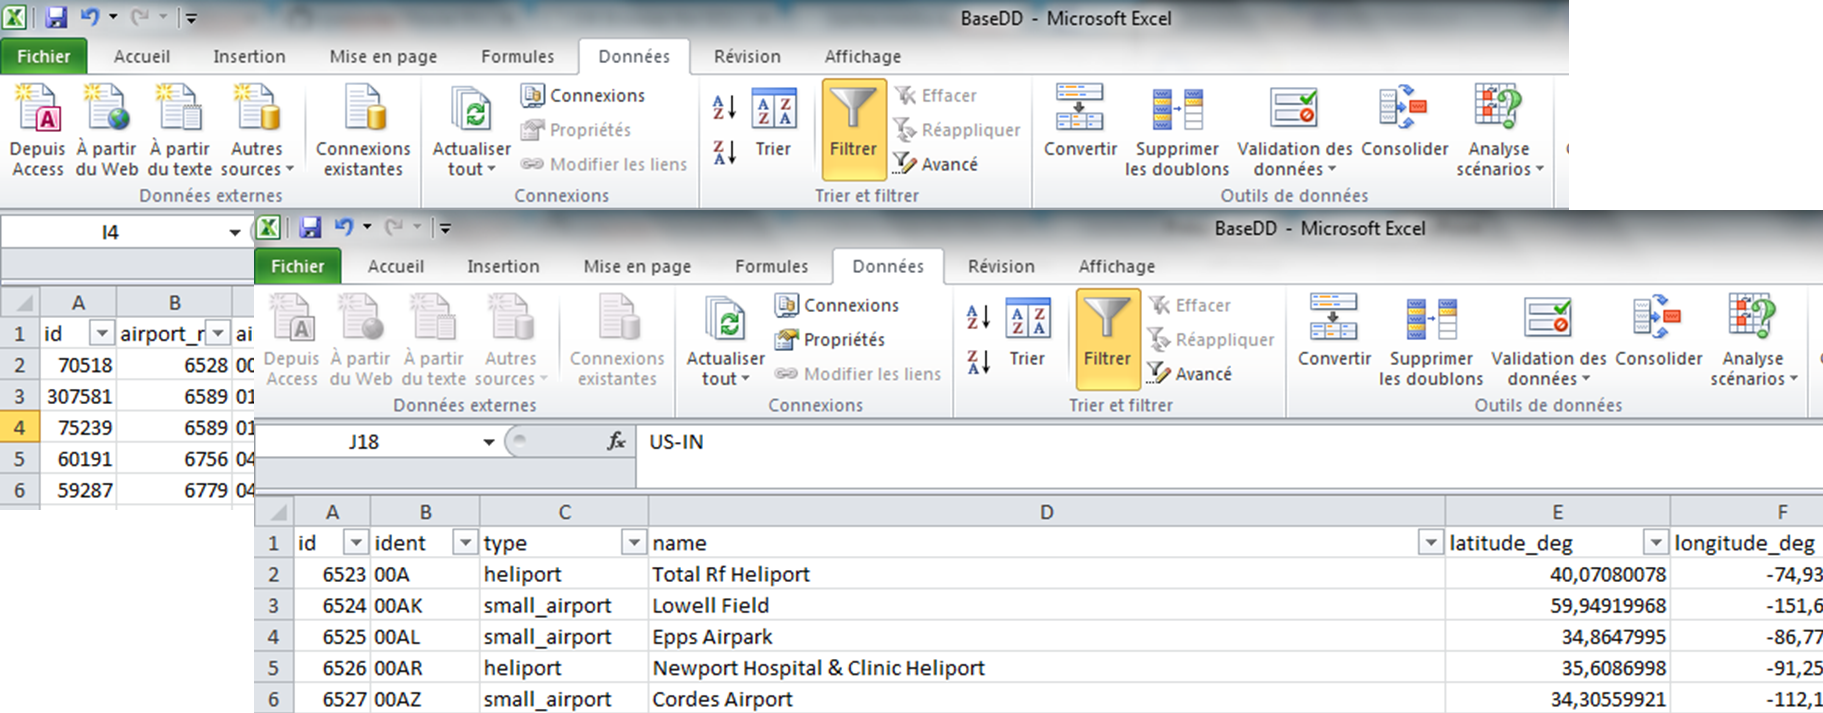
\includegraphics[width=.95\textwidth]{images/BDD_aplat}
\end{minipage}

Les bases de données sont omniprésentes dans l'industrie en général et il s'agit de présenter comment ces données sont traitées. 

On peut commencer par recenser des bases de données libres. Musicbrainz ou freedb sont par exemples des bases de données qui recensent des informations sur les disques de musiques (Auteurs, compositeurs, interprètes, titres des albums, titres des chansons, dates de sorties ...). IMDb est une base de donnée cinématographique. OpenStreetMap met à disposition des internautes des données cartographiques. 

La FNAC, ou d'autres sites commerciaux disposent d'une base de données de leurs produits. Ainsi, grâce à un champ de recherche, l'internaute peut interroger la base. Il peut avoir des informations sur la disponibilité d'un produit, le délai de livraison ...

Une organisation des données permet aux utilisateurs d'avoir un accès rapide à tout type d'informations. On appelle requête la demande d'un utilisateur formulée auprès d'une base de donnée. 

\subsection{Bases de données à <<plat>>}
Une première solution envisageable pour stocker des données est l'utilisation de bases de données dites plates. Les informations sont par exemple stockées dans un tableau. Prenons par exemple une base de données contenant la liste des aéroports du monde ainsi que diverses informations : 
\begin{center}
\begin{tabular}{p{4cm}llll}
\hline
Nom & Ville & Pays & Continent  & Type \\
\hline
\hline
Biarritz-Anglet-Bayonne Airport & Biarritz/Anglet/Bayonne & France & Europe & medium\_airport \\
Milhaud Heliport & Toulon & France & Europe & heliport \\
Toulon-Hyères Airport & Toulon/Hyères/Le Palyvestre & France & Europe & medium\_airport \\
Lake Hood Seaplane Base & Anchorage & États-Unis & Amérique du Nord & seaplane\_base\\
Ted Stevens Anchorage International Airport & Anchorage & États-Unis & Amérique du Nord & large\_airport\\
Mandalay International Airport & Mandalay & Myanmar & Asie & large\_airport\\
\hline
\end{tabular}
\end{center}

Plusieurs remarques peuvent déjà être formulées : 
\begin{itemize}
\item plusieurs informations sont stockées à plusieurs reprises : ainsi, l'information <<France>> est stockée à multiple reprise. Il en est de même pour le champ Continent;
\item des couples d'informations sont redondants : le couple (Pays, Continent) sera toujours identique pour un pays donné. Ainsi, stocker une seule fois que les États-Unis sont en Amérique du Nord.
\end{itemize}

Dans le cas d'une telle table, des requêtes simples sont aisées. Ainsi, faire la liste de tous les aéroports français ne pose pas de problème. Faire la liste de tous les héliports français est un peu plus difficile. 

Si maintenant une seconde table comprend l'ensemble des fréquences sur lesquelles chacun des aéroports peut communiquer, les tables à plat vont rapidement trouver leur limite. 

Enfin, lorsque les bases de données deviennent importantes (on recense plus de 40 000 installations aéroportuaires), l'accès aux données situées dans un tableau peut devenir considérablement lent. 

\subsection{Système de Gestion de Base de Données -- SGBD}
Pour stocker les données, on utilise des systèmes de gestion de base de données (SGBD). Le marché des SGBD est dominé par les entreprises Oracle, IBM ou Microsoft. Il existe par ailleurs des solutions libres telles que PostgreSQL ou MySQL. 

Une SGBD permettent d'assurer le stockage et l'organisation des informations ainsi que les gestions d'accès par des utilisateurs ayant des droits différents. La quantité de données peut dépasser plusieurs TéraOctets.


\subsection{Structure client -- serveur}


Classiquement, les données ne sont pas stockées sur l'ordinateur de l'utilisateur (appelé client) utilisant la base de données mais sur un serveur, voire même un <<nuage>> (\textit{cloud computing}). 

Pour simplifier, pour faire du (\textit{cloud computing}) les entreprises répartissent les informations sur plusieurs ordinateurs en réseau. Suivant les performances nécessaires ou suivant la quantité de stockage nécessaire, la base de donnée peur donc être répartie sur plusieurs ordinateurs physiques, la limite de répartition pouvant être modifié dynamiquement en fonction du besoin. 

L'architecture classique d'un site web est l'architecture trois tiers : 
\begin{center}
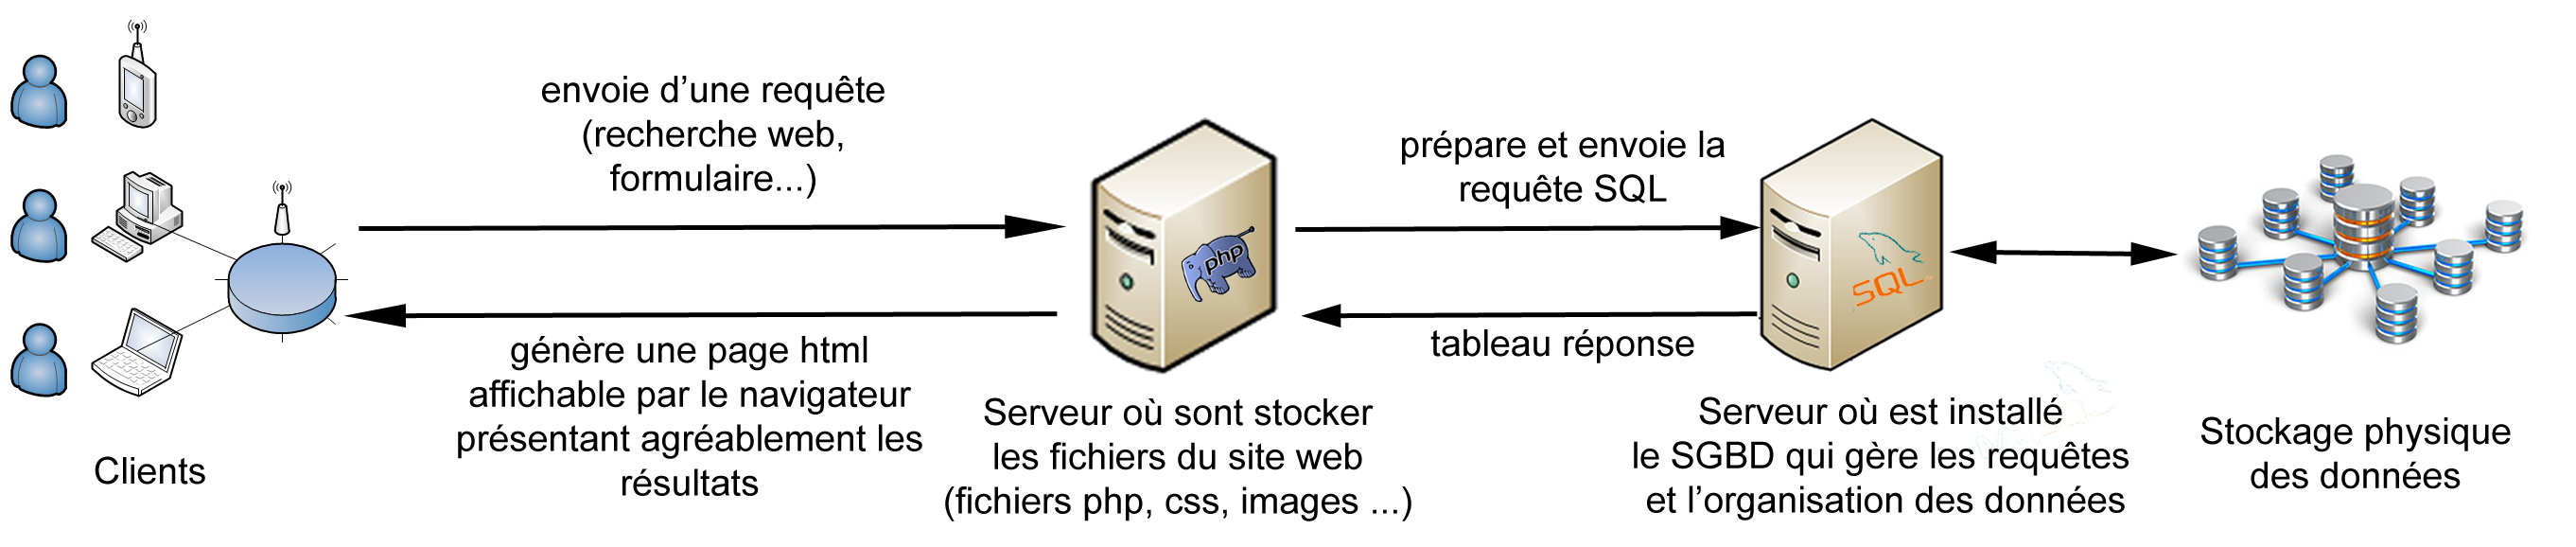
\includegraphics[width=.9\textwidth]{images/bdd}
\end{center}

\section{Structure des base de données : le modèle relationnel}
\subsection{Tables}
Dans une première approche, une base de données est constituée de tables. Une table est elle-même constituée de lignes rassemblant les informations (valeurs) que l'on désire stocker. On appellera entité chacune des lignes de cette table. Lorsque les valeurs d'une ligne ont les même propriétés, on les regroupe par colonnes. 

Lors de la conception de la base de données, on définit, pour une table, chacune des colonnes. On peut alors renseigner chacune des lignes. 

\begin{exemple}
Base de données des installations aéroportuaires
\begin{center}
\begin{tabular}{lp{4cm}p{3cm}ll}
\hline
\multicolumn{5}{c}{Aéroports} \\
\hline
Identifiant & Nom & Ville & iso\_country & Type \\
\hline
\hline
4077 &Biarritz-Anglet-Bayonne Airport & Biarritz / Anglet / Bayonne & FR &  medium\_airport \\
43537 &Milhaud Heliport & Toulon & FR  & heliport \\
4241 &Toulon-Hyères Airport & Toulon/Hyères/Le Palyvestre & FR &  medium\_airport \\
21567 &Lake Hood Seaplane Base & Anchorage & US &   seaplane\_base\\
5388 &Ted Stevens Anchorage International Airport & Anchorage & US & large\_airport\\
26727 &Mandalay International Airport & Mandalay & MM  & large\_airport\\
\hline
\end{tabular}
\end{center}

\begin{center}
\begin{tabular}{lll}
\hline
\multicolumn{3}{c}{Pays} \\
\hline
Identifiant & Code & Nom \\
\hline
\hline
302 687 & FR & France \\
302 649 & MM & Myanmar \\
302 755 & US & United States \\
\hline
\end{tabular}
\end{center}
\end{exemple}

\begin{rem}
Dans une table il n'y a pas de notion d'ordre a priori. Les données d'une ligne ne peuvent donc pas être désignées par un numéro de ligne.
\end{rem}
%
%\subsection{Définitions \cite{2}}
%
%\begin{defi}
%\textbf{Attributs -- Domaines}
%
%On considère donné un ensemble infini $\mathcal{A}$, dont les éléments sont appelés des attributs, un ensemble $D$, et une application dom de $\mathcal{A}$ dans les sous-ensembles de $D$. 
%
%Si $A\in \mathcal{A}$, $dom(A)$ est appelé domaine de $A$.
%
%\end{defi}
%
%\begin{exemple}
%Le type d'aéroport est un attribut. Son domaine est l'ensemble des types d'aéroport. 
%
%La ville est un attribut. Son domaine est l'ensemble des villes du monde muni d'un équipement aéroportuaire. 
%
%\end{exemple}
%
%\begin{defi}
%\textbf{Schéma relationnel}
%
%Un schéma relationnel est un $n$-uplet de la forme $S=(A_1,...,A_n) \in \mathcal{A}^n$ où les $A_i$ sont distincts deux à deux. 
%\end{defi}
%
%\begin{exemple}
%La table des aéroports est un schéma relationnel. 
%Sous une forme formelle, on pourrait noter :
%$$ \text{Aeroport} = \left(\left( \text{Identifiant}, \mathbb{N}\right),\left(\text{Ville}, \left( ...\right)\right), \left(\text{iso\_country},\left(\text{FR},\text{US},... \right)  \right),... \right)$$
%\end{exemple}
%
%\begin{defi}
%\textbf{Relation -- table}
%
%On appelle relation associé à un schéma relationnel $\left(A_i,...,A_n \right)$ est un ensemble fini de $n$-uplets de $dom(A_1)\times \cdot\cdot\cdot \times dom(A_n)$.
%
%On note $R(S)$ la relation $R$ pour signifier qu'elle est associée au schéma relationnel $S$. 
%
%Les éléments de $R$ sont appelés les \textit{valeurs}, ou encore les enregistrements, de la relation et leur nombre est appelé son \textit{cardinal} et est note \#R.
%\end{defi}
%
%\begin{exemple}
%Les tables présentées précédemment sont des relations. 
%\end{exemple}
%
%\begin{defi}
%\textbf{Valeurs}
%
%Si $e\in R(S)$ et $A\in S$, on note $e.A$ la composante du $n$-uplet $e$ associée à l'attribut $A$. 
%
%$R$ étant un ensemble, deux valeurs distinctes $e$ diffèrent forcément au moins sur un attribut.  Formellement, on a : 
%$$
%\forall e,e' \in R(S), \text{ si } e\neq e', \text{ alors } \exists A \in S, e.A \neq e'.A
%$$
%
%\end{defi}

\subsection{Notion de clef}
Afin de ne pas stocker des des doublons dans une base de donnée, on a recours au concept de clef primaire. 

Dans certains cas, si on est certain que la valeur d'un attribut sera différent pour chaque ligne de la table, cet attribut peut tenir compte de clef primaire. Dans d'autres cas, si on est persuadé que pour une ligne donnée, la combinaison de $n$ attributs est unique, la combinaison de ces attributs peut constituer une clef primaire. 

Enfin, dans certains cas, on définit un attribut de type <<identifiant>>. Lorsqu'on ajoute une ligne dans la table, on s'assure qu'un identifiant unique (un nombre entier par exemple) sera affecté.

\subsection{Création de base de données en langage SQL}
Le SQL (\textit{Structured Query Language}) est un langage informatique permettant :
\begin{itemize}
\item de créer des bases de données;
\item d'interroger des bases de données.
\end{itemize}

Parmi les possibilités pourinterroger une base de donnée au format SQL on peut citer les interfaces graphiques qui vont permettre d'interroger une base de donnée avec le langage naturel. Il est aussi possible d'utiliser le langage SQL directement pour faire des opérations sur une base. 

\begin{exemple}
Ainsi, il existe des API (\textit{Application Programming Interface} -- Interface de programmation) dans de nombreux langages de programmation, dont le Python, qui permettent de se connecter à une base de données et à l'interroger. 

\end{exemple}

\begin{rem}
De manière classique, les instructions SQL sont saisies en majuscules. Les requêtes se terminent par des points-virgules.
\end{rem}

\subsubsection{Création d'une base de données}


\begin{envsql}
Pour créer une base de données en langage SQL, la syntaxe est la suivante :

\begin{sql}
CREATE DATABASE Aeroports;
\end{sql}
\end{envsql}

Il est à noter qu'il existe une gestion des utilisateurs et de leurs droits. La façon la plus aisée de les gérer est d'utiliser une interface graphique (par exemple phpmyadmin avec des bases de type mysql).

\subsubsection{Création d'une table}
Une fois la base de données crée, il est nécessaire de créer les tables. Chaque table dispose d'un ou de plusieurs attributs. Il existe plusieurs types d'attributs parmi lesquels : 
\begin{itemize}
 \item des entiers entiers. Il en existe plusieurs types selon les nombres à stocker (de \texttt{TINYINT} (codé sur un octet) et ayant une capacité de -128 à 127 à \texttt{BIGINT} (codé sur 8 octets));
 \item la date et l'heure, permettant de stocker par exemple l'heure (\texttt{TIME} au format HH:MM:SS) ou l'année (\texttt{YEAR} au format AAAA).
 \item du texte : \texttt{CHAR} permet de stocker jusqu'à 255 caractères.
 \item \textit{etc}.
\end{itemize}

\begin{envsql}

Ainsi, pour créer une table, on a recours à la syntaxe suivante :
\begin{sql}
CREATE TABLE nom_table (nom_attribut_1 type_attribut1, nom_attribut_2  type_attribut_2, ...);
\end{sql}
\end{envsql}

\begin{exemple}
Étant dans la base de données Aéroports, pour créer la table des pays avec comme attributs un identifiant (de type entier), un code (de type chaîne de caractères) un nom (de type chaîne de caractères), on a :
\begin{envsql}
\begin{sql}
CREATE TABLE Pays (Identifiant INT, Code CHAR, Nom CHAR);
\end{sql}
\end{envsql}

\end{exemple}

Lors de la création des tables il est de plus possible de définir des contraintes :
\begin{itemize}
\item \texttt{NOT NULL} : empêche d'avoir un 0 dans un champ;
\item \texttt{UNIQUE} : permet de n'avoir aucun doublon dans une colonne;
\item \texttt{DEFAULT} permet d'attribuer une valeur par défaut lorsque le champ n'est pas défini lors de l'insertion d'un élément;
\item \texttt{PRIMARY KEY} permet de définir un attribut comme clef primaire;
\item \textit{etc}.
\end{itemize}

\begin{exemple}
Pour la même table que précédemment, il est possible de déclarer que l'identifiant est une clef unique primaire dont les occurrences sont uniques. On impose que le code et le nom des aéroports soient obligatoirement renseignés.


\begin{envsql}
\begin{sql}
CREATE TABLE Pays (Identifiant INT UNIQUE PRIMARY KEY , Code CHAR NOT NULL , Nom CHAR NOT NULL);
\end{sql}
\end{envsql}
\textit{Remarque : } Le code d'aéroport étant un code unique, il devrait normalement être inutile d'avoir un identifiant. La clef primaire pourrait alors être le code. 

\end{exemple}

\subsection{Suppléments}
Il est possible de supprimer une table, une base de données, de modifier la structure d'une table...
\section{Algèbre relationnelle}
La raison d'être d'une base de données étant de disposer de données, il est nécessaire de disposer d'outils d'interrogation. Pour cela, il existe un mathématique formel appelé algèbre relationnelle. Chaque opération formelle est transposable dans un langage de programmation. 





\begin{defi}
\textbf{Requêtes -- Algèbre relationnelle}

On entend par algèbre relationnelle, une collection d'opérations (requêtes) formelles qui agissent sur des relations et produisent une relation en résultat : $R_3 \leftarrow R_2 Op R_1$.
\end{defi}

Ceci signifie que dans l'algèbre relationnelle, le résultat des requêtes effectuées sur les relations (tables) sera toujours une nouvelle relation. 
%
%\begin{rem}
%\textit{Sélection des éléments d'une table}
%
%Pour sélectionner tous les éléments d'une table, on utilise la requête suivante : 
%\begin{envsql}
%\begin{sql}
%SELECT * FROM nom_table;
%\end{sql}
%\end{envsql}
%
%Pour sélectionner seulement certains attributs d'une table, on utilise la requête suivante : 
%\begin{envsql}
%\begin{sql}
%SELECT attribut_1,attribut_2 FROM nom_table;
%\end{sql}
%\end{envsql}
%
%\end{rem}


\subsection{Opérations relationnelles}
\subsubsection{Projection}

\begin{defi}

\textbf{Projection}

Opération notée $\pi$ au cours de laquelle on sélectionne certaines des colonnes (on élimine donc des attributs). 
\ifprof

$$
 R_2 \leftarrow \pi_{\text{attribut 1, attribut 2, ...}}(R_1)
$$

\else
$$ \quad $$
$$ \quad $$
\fi

\ifprof
\begin{envsql}
\begin{sql}
SELECT attribut_1,attribut_2 FROM nom_table;

SELECT * FROM nom_table;
\end{sql}
\end{envsql}
\else
\begin{envsql}
\begin{sql}
. 
 

.
\end{sql}
\end{envsql}
\fi
\end{defi}

\begin{exemple}
Lister les noms d'aéroports ainsi que les codes IATA correspondant :

\ifprof
$$
\pi_{\text{name,iata\_code}}(\text{airports})
$$

\begin{envsql}
\begin{sql}
SELECT name,iata_code FROM airports
\end{sql}
\end{envsql}
\else

\vspace{3cm}

\fi
\end{exemple}

\subsubsection{Sélection}
\begin{defi}
\textbf{Sélection}

On appelle sélection de $R_1$ selon $A=a$, et on note $\sigma_{A=a}(R_1)$, la relation obtenue en sélectionnant dans $R_1$ uniquement les valeurs $e$ telles que $e.A = a$.
\ifprof

$$
R_2 \leftarrow \sigma_{\text{attribut}=\text{condition}}(R_1)
$$

\else
$$
\quad
$$
$$
\quad
$$
\fi

Le schéma relationnel $R_2$ est identique au schéma $R_1$.  Les opérateurs permettant d'exprimer une condition sont $=$, $\neq$ (\texttt{!=} ou \texttt{<>}), $<$, $\leq$ (\texttt{<=}), $\geq$ (\texttt{>=}), $\neg$ (négation, \texttt{NOT}), $\vee$ (ou, \texttt{OR}), $\wedge$ (et, \texttt{AND}).

\begin{envsql}
\begin{sql}
SELECT att_1,att_2 FROM nom_table WHERE att_3="xx" AND att_4=0 ...
\end{sql}
\end{envsql}

\end{defi}

\begin{exemple}
Sélectionner le nom de tous les aéroports situés au niveau de la mer :

\ifprof
$$
\pi_{\text{name}}\left(\sigma_{\text{elevation\_ft = 0}}(\text{airports})\right)
$$
\begin{envsql}
\begin{sql}
SELECT name FROM airports WHERE elevation_ft=0
\end{sql}
\end{envsql}
\else
\vspace{3cm}
\fi

Sélectionner le nom et le code iata de tous aéroports situés en-dessous du niveau de la mer en Europe :
\ifprof
$$
\pi_{\text{name},\text{iata\_code}}\left(\sigma_{\text{elevation\_ft} < \text{0}\wedge \text{continent}=\text{EU})}(\text{airports} )\right)
$$
\begin{envsql}
\begin{sql}
SELECT name,iata_code FROM airports WHERE elevation_ft<0 AND continent="EU";
\end{sql}
\end{envsql}
\else
\vspace{3cm}
\fi


Cette requête laisse apparaître 2 fois la même ligne : 
\begin{sql}
Mashland Airfield   
\end{sql}
Cela s'explique par le fait que l'aéroport apparait 2 fois dans la table airports. Mais, pour la liste d'attributs sélectionnés, tous les champs sont les mêmes (l'identifiant est bien différent). En faisant apparaître l'id, on réaliserait que les deux champs sont différents. 
Si on souhaite éliminer les doublons dans, la requête est la suivante : 

\begin{envsql}
\begin{sql}
SELECT DISTINCT name,iata_code FROM airports WHERE elevation_ft<0 AND continent="EU";
\end{sql}

\end{envsql}

\end{exemple}


\subsubsection{Renommage}
\begin{defi}
\textbf{Renommage d'attribut}

Cette opération est utilisée pour des raisons pratiques pour lever une ambigüité ou pour simplifier le nom d'un attribut de façon temporaire. 

Soit $S = (A_1,... ,A_n)$ un schéma, $ i \in[1;n]$ et $B$ un attribut tel que
$dom(B) = dom(A_i)$. On note :

$$
R_2 (S)\leftarrow \rho_{\text{ancien attribut} \rightarrow \text{nouvel attribut}}(R_1(S))
$$

\begin{envsql}
\begin{sql}
SELECT att_1,att_2 as att_3 FROM nom_table
\end{sql}
\end{envsql}

\end{defi}


\begin{exemple}
On désire sélectionner le nom des aéroports et les altitudes et  renommer temporairement l'attribut \texttt{elevation\_ft} en \texttt{altitude} :
\ifprof
$$
\pi_{\text{elevation\_ft}}\left(\rho_{\text{elevation\_ft} \rightarrow \text{altitude}}(\text{airports})\right)
$$
\begin{envsql}
\begin{sql}
SELECT name, elevation_ft AS altitude FROM airports;
\end{sql}
\end{envsql}
\else
\vspace{3cm}
\fi

\end{exemple}




\subsection{Opérations sur les ensembles}
\begin{rem}
Les opérateurs ensemblistes sont dédiés à des relations de même schéma relationnel. 
\end{rem}


\subsubsection{Opérations cartésiennes}

\begin{defi}

\textbf{Produit cartésien}

Soient $R_1(S_1)$ et $R_2(S_2)$ deux relations de schémas disjoints. L'opération produit cartésien est notée $\times$. 

$$
R_3 \leftarrow R_1 \times R_2
$$

La relation $R_3$ contient toutes les combinaisons d'association possibles entre les valeurs de $R_1$ et de $R_2$.

\begin{envsql}
\begin{sql}
SELECT * FROM table_1,table_2
\end{sql}
\end{envsql}

\end{defi}



\begin{defi}

\textbf{Division cartésienne}

Soient $R_1(S_1)$ et $R_2(S_2)$ deux relations de schémas disjoints. L'opération division cartésienne est notée $\div$. 

$$
R_3 \leftarrow R_1 \div R_2
$$

Dans ce cas, toutes les combinaisons de chaque tuple de $R_3$ et de chaque tuple de $R_2$ est contenue dans $R_1$.

\end{defi}


\begin{exemple}
On désire sélectionner les continents qui ont tous types d'aéroports :
$$
\pi_{\text{name}}\left(\text{airports} \div \pi_{\text{type}}\left( \text{airports})\right)\right)
$$

Il n'y a pas de transcription en langage SQL.
\end{exemple}



\subsubsection{Union}

\begin{defi}
\begin{minipage}[c]{.75\linewidth}
\textbf{Union}

L'union de deux relations $R_1(S)$ et $R_2(S)$ est l'ensemble des valeurs comprises dans $R_1$ ou $R_2$. 

On peut donc noter la relation $R_3(S)$ définie par : $R_3(S)\leftarrow R_1(S)\cup R_2(S)$
\end{minipage}\hfill
\begin{minipage}[c]{.2\linewidth}
\begin{center}
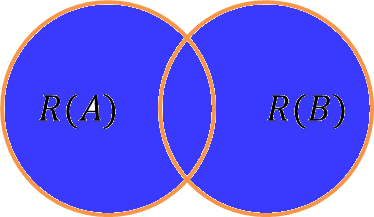
\includegraphics[width=.95\textwidth]{images/union}
\end{center}
\end{minipage}

\end{defi}

\begin{envsql}
En langage SQL pour pouvoir faire l'union de deux relations, elles doivent avoir le même schéma (même nombre de colonne(s) et même type de colonnes). Il faut prêter attention à l'ordre des attributs dans la requête. 

\begin{sql}
SELECT  attribut_11, attribut_12 FROM table_1 UNION attribut_21, attribut_22 FROM table_2
\end{sql}
\end{envsql}

\begin{exemple}
Ainsi, pour connaître les noms des régions et des pays associés à leur code, on utilise la requête suivante :

\ifprof
\begin{envsql}
\begin{sql}
SELECT code,name FROM Countries UNION SELECT code,name FROM Regions;
\end{sql}
\end{envsql}
\else
\vspace{3cm}
\fi

La relation résultant contient donc l'ensemble des couples (code,name) des régions et des  pays. 
\end{exemple}

\begin{rem}
Cette opération est à utiliser avec attention car la relation résultante peut avoir une forme absurde.
\end{rem}

\subsubsection{Intersection}
\begin{defi}
\begin{minipage}[c]{.75\linewidth}
\textbf{Intersection}

L'intersection de deux relations $R_1(S)$ et $R_2(S)$ est l'ensemble des valeurs comprises dans $R_1$ et dans $R_2$. 

On peut donc noter la relation $R_3(S)$ définie par : $R_3(S)\leftarrow R_1(S)\cap R_2(S)$

\begin{envsql}
\begin{sql}
SELECT  (expression 1) INTERSECT SELECT (expression 2);
\end{sql}
\end{envsql}
\end{minipage}\hfill
\begin{minipage}[c]{.2\linewidth}
\begin{center}
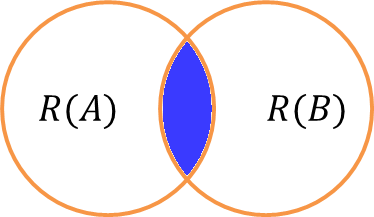
\includegraphics[width=.95\textwidth]{images/inter}
\end{center}
\end{minipage}
\end{defi}

\begin{exemple}
Sélectionner le nom de l'ensemble des aéroports européens dont l'altitude est en dessous du niveau de la mer :
\ifprof
$$
\pi_{\text{name}}\left(\sigma_{\text{continent}=''EU''}(\text{airports}) \cap \sigma_{\text{elevation\_ft}\leq0}(\text{airports}) \right)
$$
\begin{envsql}
\begin{sql}
SELECT name FROM airports WHERE continent=''EU''
    INTERSECT SELECT name FROM airports WHERE elevation_ft<=0;
\end{sql}
\end{envsql}
\else
\vspace{4cm}
\fi

\end{exemple}


\subsubsection{Différence}
\begin{defi}
\begin{minipage}[c]{.75\linewidth}
\textbf{Différence}

La différence de deux relations $R_1(S)$ et $R_2(S)$ est l'ensemble des valeurs comprises dans $R_1$ et qui ne sont pas comprises dans $R_2$. 

On peut donc noter la relation $R_3(S)$ définie par : $R_3(S)\leftarrow R_1(S)-R_2(S)$

\begin{envsql}
\begin{sql}
SELECT  (expression 1) EXCEPT SELECT (expression 2);
\end{sql}
\end{envsql}

\end{minipage}\hfill
\begin{minipage}[c]{.2\linewidth}
\begin{center}
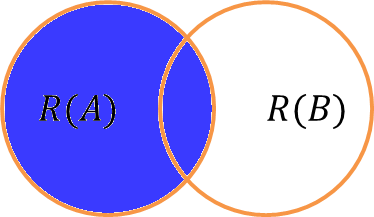
\includegraphics[width=.95\textwidth]{images/diff}
\end{center}
\end{minipage}
\end{defi}

\subsubsection{Jointures}

\begin{defi}

\textbf{Jointure}

La jointure est une combinaison de de tuples de deux relations en un seul tuple. On ne s'intéresse ici qu'à la jointure symétrique simple qui permet de recoller deux relations ayant un attribut en commun. 

$$ 
R_3 \leftarrow \sigma_{\text{R1.attribut\_1=R2.attribut\_2}} (R_1\times R_2) \quad \quad 
R_3 \leftarrow \underset{\text{R1.attribut\_1=R2.attribut\_2}}{R_1 \bowtie R_2}
$$

\begin{envsql}
\begin{sql}
SELECT att_1,... FROM table_1 JOIN table_2 ON attribut.R1=attribut.R2
\end{sql}
\end{envsql}

\end{defi}

\begin{exemple}
Dans la table airrpots, les pays sont référencés par un attribut nommé iso\_country. La table Countries fait le lien entre l'attribut code et l'attribut name. 

L'utilisateur ne connaissant pas le code pays, il souhaite en une seule requête connaître la liste de tous les aéroports français. 
\ifprof
%$$
%\pi_{\text{name}}\left( 
%\sigma_{\text{airports.iso\_country}=\text{Countries.code}}\left(
%\text{Countries} \times \text{airports}
%\right)
%\right)
%$$
$$
\pi_{\text{name}}\left( 
\pi_{\text{name,code}}\left(\text{Countries}  \right)
\underset{\text{airports.iso\_country}=\text{Countries.code}}{\bowtie }
\pi_{\text{name,iso\_country}}\left( \text{airports}  \right)
\right)
$$

\begin{envsql}
\begin{sql}
SELECT name FROM 
    (SELECT name, iso_country FROM airports) AS aeroports
    INNER JOIN 
    (SELECT Countries.code from Countries WHERE name="France") AS pays     
        ON aeroports.iso_country=pays.code
\end{sql}
\end{envsql}
\else
\vspace{6cm}
\fi


\end{exemple}

\subsection{Fonctions d'agrégations}
\begin{defi}
Ces fonctions qui ne sont pas couvertes par l’algèbre relationnelle 
classique, permettent d’effectuer des calculs statistiques basiques sur les valeurs : \texttt{MIN}, \texttt{MAX}, \texttt{SUM} 
(somme), \texttt{AVG} (moyenne), \texttt{COUNT} (comptage du nombre de lignes). 

\end{defi}


\begin{exemple}
\textit{Combien existe-t-il d'aéroports en France ?}

\begin{envsql}
\begin{sql}
SELECT COUNT(airports.name) 
        FROM airports 
    INNER JOIN 
        (SELECT Countries.code from Countries WHERE name="France") as pays 
    ON airports.iso_country=pays.code
\end{sql}
\end{envsql}

\textit{Quel est l'aéroport le plus élevé ?}
\begin{envsql}
\begin{sql}
SELECT MAX(elevation_ft) FROM 
    (SELECT elevation_ft, name, iso_country FROM airports WHERE elevation_ft!='''') AS aeroports
    INNER JOIN 
    (SELECT Countries.code from Countries WHERE name="France") AS pays     
        ON aeroports.iso_country=pays.code
\end{sql}
\end{envsql}

\textit{Quel est l'aéroport le plus élevé en mètres ?}
\begin{envsql}
\begin{sql}
SELECT MAX(elevation_ft)*0.30478513 FROM 
    (SELECT elevation_ft, name, iso_country FROM airports WHERE elevation_ft!='''') AS aeroports 
    INNER JOIN 
    (SELECT Countries.code from Countries WHERE name="France") as pays 
        ON aeroports.iso_country=pays.code
\end{sql}
\end{envsql}

\end{exemple}
\newpage


\begin{rem}
Formalisme général de l’instruction SQL « SELECT » :
\begin{envsql}
\begin{sql}
SELECT <liste d expressions> 
    FROM <liste de tables> 
    WHERE <conditions> 
    GROUP BY <liste d attributs> 
    HAVING <conditions> 
    ORDER BY <liste d attributs> 
\end{sql}
\end{envsql}
\end{rem}

\begin{thebibliography}{2}
\bibitem{1}{Serge Abiteboul, Benjamin Nguyen, Yannick Le Bras, \textit{Introduction aux Bases de Données Relationnelles Programme de Classes Préparatoires Scientifiques, Première année}.}
%\bibitem{2}{Wack et Al., \textit{L’informatique pour tous en classes préparatoires aux grandes écoles, Editions Eyrolles}.}
\bibitem{3}{Christope Revy, \textit{Concepts des bases de données}, Cours de STS IRIS, Lycée Janot de SENS.}
\bibitem{4}{Patrick Beynet, \textit{Supports de cours de TSI 2}, Supports de cours de TSI 2, Lycée Rouvière, Toulon.}
\bibitem{5}{\url{http://sqlpro.developpez.com/cours/divrelationnelle/}}
\end{thebibliography}
\end{document}


